\section{Aktuator} \label{sec:AktImpl}

Dette afsnit beskriver implementering af SW og HW i blokken Aktuator. Afsnittet beskriver først hhv. HW og SW i underblokken PSoC4, herefter HW i underblokkene Varmelegeme, Blæsere og Vinduesmotor.

\subsection{HW PSoC4}
\begin{figure}[h]
\centering 
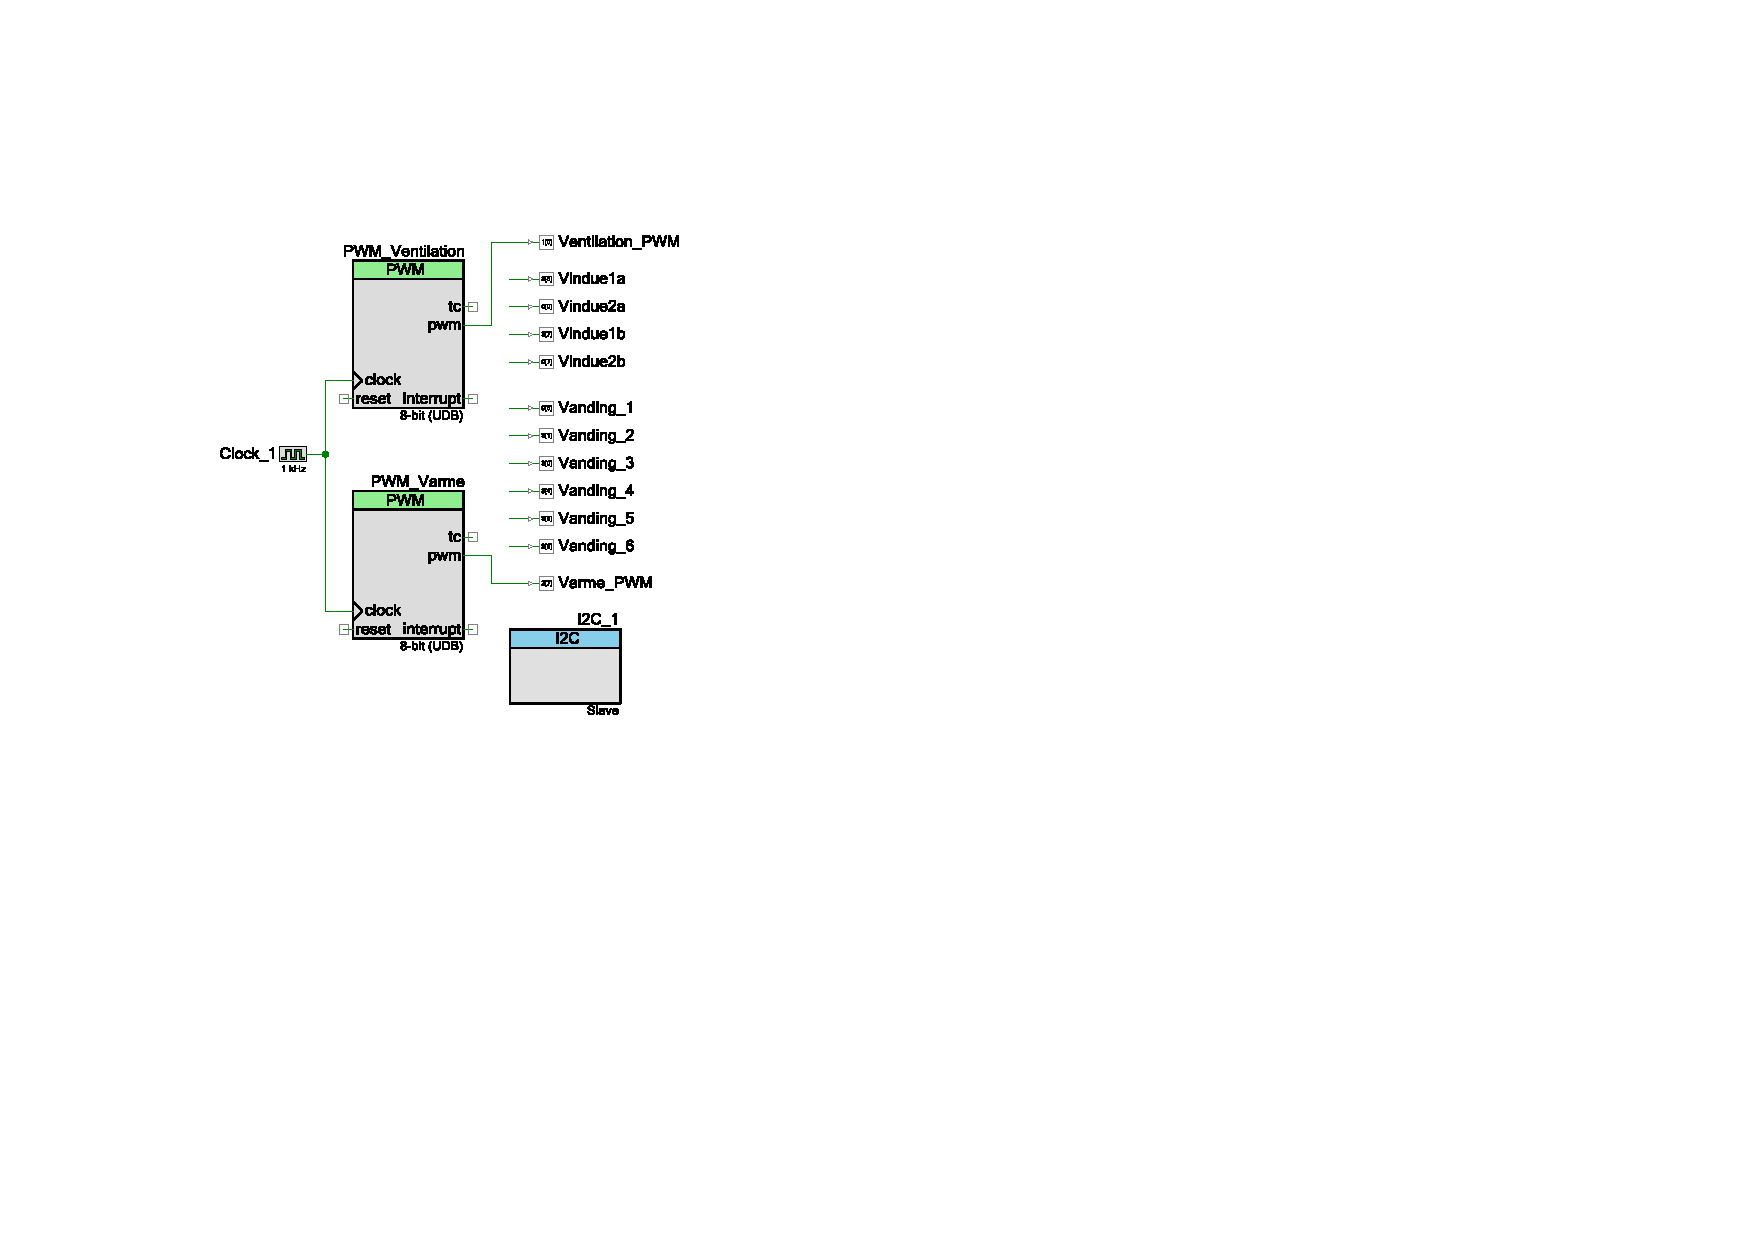
\includegraphics[width={\textwidth-6cm}, trim = 110 320 480 100, clip=true] {../fig/TopDesign_Aktuator.pdf}
\caption{TopDesign.cysch for PSoC4 i Aktuator}
\label{fig:topdesign_aktuator}
\end{figure}

Den HW, der syntetiseres i PSoC4 Aktuator er vist på figur\ref{fig:topdesign_aktuator}. 

Clock\_1 forsyner PWM komponenten med en grundfrekvens; der er valgt 1 kHz.

PWM\_Ventilation genererer et PWM signal til styring af drivhusets fire ventilatorer. Timeren er indstillet til 8 bit.  

I2C\_1 komponenten styrer kommunikation med MasterPSoC via \IIC. 
Den konfigureret til at være slave med adressen 0x42, datarate er indstillet til 100 kbps.

Alle pins i topdeignet er konfigureret til strong drive. 
Det vil sige at de altd er defineret enten high eller low.

\clearpage

\subsection{SW PSoC4}

\begin{lstlisting}[caption=Udsnit af main.c for PSoC4 i Aktuator, label=fig:main_aktuator]
    for(;;) //Evigt loop
    {
        checkForData(); //Opdater Status_Reg, hvis der er modtaget data
        
        if(!(Status_Reg == Position_Reg))//Hvis der er et mismatch
        {
            //Tjek for mismatch for Varme
            if(!((Status_Reg & 0b0000111000000000) == (Position_Reg & 0b0000111000000000)))
            {
                AdjustHeat();
            }
            
            //Tjek for mismatch for Ventilation
            if(!((Status_Reg & 0b0000000111000000) == (Position_Reg & 0b0000000111000000)))
            {
                AdjustVentilation();
            }
            
            //Tjek for mismatch for Vanding
            if(!((Status_Reg & 0b0000000000111111) == (Position_Reg & 0b0000000000111111)))
            {
                AdjustIrrigation();
            }
            
            //Tjek for mismatch for Vindue
            if(!((Status_Reg & 0b1111000000000000) == (Position_Reg & 0b1111000000000000)))
            {
                AdjustWindow();
            }
        }
    }
\end{lstlisting}

Filen main.c, hvoraf den vigtigste del er vist på Listing \ref{fig:main_aktuator}, fungerer jf. State Machinen på Figur \ref{fig:stm_psoc_aktuator} side \pageref{fig:stm_psoc_aktuator}.

Programmet tjekker om der er modtaget data på \IIC, og opdaterer evt. ønskede indstillinger for aktuatorer i Status\_Reg. 

Herefter sammenlignes Status\_Reg med nuværende indstillinger af aktuatorer i Position\_Reg.

Såfremt der er uoverensstemmelse, opdateres den pågældende aktuator. 

Sammenligningen af de to registre sker i en prioriteret rækkefølge. 

Vinduet er sidste i denne proces, da det tager temmelig lang tid (flere sekunder) at åbne eller lukke vindet. 

\clearpage

\begin{lstlisting}[caption=Udsnit af checkForData.c for PSoC4 i Aktuator, label=fig:checkForData_aktuator]
void checkForData()
{
    uint16 temp = 0;
    //Check for om der er modtaget data
    if(I2C_1_I2CSlaveStatus() & I2C_1_I2C_SSTAT_WR_CMPLT)
    {
        //Put data i Status_Reg            
        if((writeBuffer[0] >> 6) == 0x0) //Check for Vindue
        {
            //Put data fra buffer i uint16 og skift til rigtig position
            temp = (writeBuffer[0] & 0b00001111) << 12; 
            //Overskriv relevante pladser med 0'er
            Status_Reg = Status_Reg & 0b0000111111111111;
            //Put nye data ind i Status_Reg
            Status_Reg = Status_Reg | temp;                
        }           
        if((writeBuffer[0] >> 6) == 0x1) //Check for Varme
        {
            //Put data fra buffer i uint16 og skift til rigtig position
            temp = (writeBuffer[0] & 0b00000111) << 9; 
            //Overskriv relevante pladser med 0'er
            Status_Reg = Status_Reg & 0b1111000111111111;
            //Put nye data ind i Status_Reg
            Status_Reg = Status_Reg | temp;                
        }           
        if((writeBuffer[0] >> 6) == 0x2) //Check for Ventilation
        {
            //Put data fra buffer i uint16 og skift til rigtig position
            temp = (writeBuffer[0] & 0b00000111) << 6; 
            //Overskriv relevante pladser med 0'er
            Status_Reg = Status_Reg & 0b1111111000111111;
            //Put nye data ind i Status_Reg
            Status_Reg = Status_Reg | temp;                
        }            
        if((writeBuffer[0] >> 6) == 0x3) //Check for Vanding
        {
            //Put data fra buffer i uint16 og skift til rigtig position
            temp = (writeBuffer[0] & 0b00111111); 
            //Overskriv relevante pladser med 0'er
            Status_Reg = Status_Reg & 0b1111111111000000;
            //Put nye data ind i Status_Reg
            Status_Reg = Status_Reg | temp;                
        }                    
        I2C_1_I2CSlaveClearWriteBuf(); //Clear buffer pointer
        I2C_1_I2CSlaveClearWriteStatus(); //Clear status                       
        //Opdater Read buffer
        readBuffer[0] = Status_Reg >> 8;
        readBuffer[1] = Status_Reg;     
        I2C_1_I2CSlaveClearReadBuf();
    }
}
\end{lstlisting}

\clearpage

Funktionen checkForData() på Listing \ref{fig:checkForData_aktuator} checker om slavens status er, at den har modtaget data. 

I så fald checker den for hvilken aktuator, der modtages data til.
Herefter behandles data, og Status\_Reg opdateres.

Efter dette klargøres systemet til at modtage nye data, ved at write buffer og status for slaven nulstilles.

Til slut opdateres read buffer, i tilfælde af at MasterPSoC beder om information om aktuel status. 
\newline
\begin{lstlisting}[caption=Udsnit af heat.c for PSoC4 i Aktuator, label=fig:heat_aktuator]
void InitHeat()
{   
    //Slukker for Varme
    Varme_Write(0);
    
    //Opdater nuvaerende indstillinger
    Position_Reg = Position_Reg & 0b1111000111111111;
}

void AdjustHeat()
{
    //Opdater aktuator for varmelegeme
    Varme_Write((Status_Reg & 0b0000111000000000) >> 9);
    
    //Opdater nuvaerende indstillinger
    Position_Reg = Position_Reg & 0b1111000111111111;
    Position_Reg = Position_Reg | (Status_Reg & 0b0000111000000000);
}
\end{lstlisting}

Koden i heat.c i Listing \ref{fig:heat_aktuator} består af to funktioner. 

InitHeat()trækker pin for varme lav og initialiserer indstilling af Position\_Reg for varme.

AdjustHeat() opdaterer pin for varme og Position\_Reg opdateres med de nuværende indtillinger for aktuator. 

\clearpage

\begin{lstlisting}[caption=Udsnit af ventilation.c for PSoC4 i Aktuator, label=fig:ventilation_aktuator]
void InitVentilation()
{
    //Start komponent
    PWM_Ventilation_Start();
    //Sluk ventilatorer
    PWM_Ventilation_WriteCompare(0);
    //Opdater nuvaerende indstillinger
    Position_Reg = Position_Reg & 0b1111111000111111;
}

void AdjustVentilation()
{
    //Start med fuld styrke for at blaeserne kommer i gang.
    PWM_Ventilation_WriteCompare((MAXIMUM_VENT*255)/100);
    CyDelay(100);
    //Omregn bits fra Status_Reg og start PWM med oensket dutycycle
    PWM_Ventilation_WriteCompare((((Status_Reg & 0b0000000111000000) >> 6)*MAXIMUM_VENT*255)/(7*100));
    
    //Opdater nuvaerende indstillinger
    Position_Reg = Position_Reg & 0b1111111000111111;
    Position_Reg = Position_Reg | (Status_Reg & 0b0000000111000000);
}
\end{lstlisting}

Koden i ventilation.c i Listing \ref{fig:ventilation_aktuator} består af to funktioner. 

InitVentilation() starter PWM komponenten, slukker for blæsere (dutycycle = 0\%) og initialiserer indstilling af Position\_Reg for ventilation.

AdjustVentilation() indstiller ønsket dutycycle i PWM komponenten. 

MAXIMUM\_VENT er en global definition af den dutycycle, der maximalt ønskes. Ved praktiske forsøg er det konstateret at 50\% er passende.

For at sikre at blæserne rent faktisk kommer i gang, startes PWM komponenten først for fuld styrke i 100 ms, hvorefter den ønskede dutycycle indstilles.

Der er som udgangspunkt kun mulighed for at tænde eller slukker for ventilationen, men ved at lave koden på denne måde, kan systemet meget nemt opgraderes, hvis PWM styring af varmelegemet ønskes. 

Efter start at PWM komponenten opdateres Position\_Reg med de nuværende indtillinger for aktuatorer.

\clearpage

\begin{lstlisting}[caption=Udsnit af irrigation.c for PSoC4 i Aktuator, label=fig:irrigation_aktuator]
void InitIrrigation()
{
    //Sluk for al vanding
    Vanding_1_Write(0);
    Vanding_2_Write(0);
    Vanding_3_Write(0);
    Vanding_4_Write(0);
    Vanding_5_Write(0);
    Vanding_6_Write(0);
    
    //Opdater nuvaerende indstillinger
    Position_Reg = Position_Reg & 0b1111111111000000;
}

void AdjustIrrigation()
{
    //Opdater alle aktuatorer for vanding
    Vanding_1_Write(Status_Reg & 0b0000000000000001);
    Vanding_2_Write((Status_Reg & 0b0000000000000010) >> 1);
    Vanding_3_Write((Status_Reg & 0b0000000000000100) >> 2);
    Vanding_4_Write((Status_Reg & 0b0000000000001000) >> 3);
    Vanding_5_Write((Status_Reg & 0b0000000000010000) >> 4);
    Vanding_6_Write((Status_Reg & 0b0000000000100000) >> 5);
    
    //Opdater nuvaerende indstillinger
    Position_Reg = Position_Reg & 0b1111111111000000;
    Position_Reg = Position_Reg | (Status_Reg & 0b0000000000111111);
}
\end{lstlisting}

Koden i irrigation.c i Listing \ref{fig:irrigation_aktuator} består af to funktioner. 

InitIrrigation() trækker alle pins for vanding lav og initialiserer Position\_Reg.

AdjustIrrigation() opdaterer alle pins for vanding og indstiller Position\_Reg.

\clearpage

\begin{lstlisting}[caption=Udsnit A af window.c for PSoC4 i Aktuator, label=fig:window1_aktuator]
void InitWindow()
{
    //Initialisering af pins til startposition
    Vindue1a_Write(1);
    Vindue2a_Write(1);
    Vindue1b_Write(0);
    Vindue2b_Write(0);
    //Initialisering af nuvaerende position
    currentTurn = 0;
    //Opdatering af nuvaerende indstillinger
    Position_Reg = Position_Reg & 0b0000111111111111;
}

void AdjustWindow()
{      
    //Konvertering af data fra Status_Reg og indsaettelse i desiredTurn.
    desiredTurn = ((MAX_WINDOW)*(((Status_Reg >> 12)*100)/15))/100;
    
    while(desiredTurn != currentTurn) //Saa laenge vinduet ikke er i oensket position
    {
        if (currentTurn > desiredTurn) //Luk 1 omgang hvis vinduet er for aabent
        {
            CloseOneTurn();
        }
    
        if (currentTurn < desiredTurn) //aaben 1 omgang hvis vinduet er for lukket
        {
            OpenOneTurn();
        }
    }
    //Opdatering af nuvaerende indstillinger
    Position_Reg = Position_Reg & 0b0000111111111111;
    Position_Reg = Position_Reg | (Status_Reg & 0b1111000000000000);
}
\end{lstlisting}

Kodeudnsnittet fra window.c på Listing \ref{fig:window1_aktuator} viser de to funktioner InitWindow() og AdjustWindow().

MAX\_WINDOW er en global definition, som angiver antallet af steps motoren skal køre, for at åbne vinduet helt. 
TIME\_BETWEEN\_STEPS er en global definition som angiver hvor mange milisekunder, der går mellem hvert af motorens steps. 
Ved praktiske forsøg er hhv. 420 steps og 10 ms fundet hensigtsmæssige.

InitWindow() initialiserer de fire vindues pins til startposition og initialiserer Position\_Reg. 

Den initialiserer desuden variablen currentTurn til 0. Denne variabel holder styr på hvor vinduet befinder sig. 

BEMÆRK! Vinduet skal være lukket, når systemet startes!

AdjustWindow() kontrollerer om currentTurn er større, mindre eller lig desiredTurn. Hvis de er forskellige kaldes enten OpenOneTurn() eller CloseOneTurn().

Herefter opdateres Position\_Reg.

\clearpage

\begin{lstlisting}[caption=Udsnit B af window.c for PSoC4 i Aktuator, label=fig:window2_aktuator]
void CloseOneTurn()//48 steps paa en omgang, 12*4=48, funktionen lukker 1/12 af en omgang.
{
    //Efter hvert fjerde step checkes der for ny data og stilling samt oenskede stilling opdateres
    Vindue1a_Write(0);
    Vindue2a_Write(1);
    Vindue1b_Write(1);
    Vindue2b_Write(0);
    CyDelay(TIME_BETWEEN_STEPS);
    Vindue1a_Write(0);
    Vindue2a_Write(0);
    Vindue1b_Write(1);
    Vindue2b_Write(1);
    CyDelay(TIME_BETWEEN_STEPS);
    Vindue1a_Write(1);
    Vindue2a_Write(0);
    Vindue1b_Write(0);
    Vindue2b_Write(1);
    CyDelay(TIME_BETWEEN_STEPS);
    Vindue1a_Write(1);
    Vindue2a_Write(1);
    Vindue1b_Write(0);
    Vindue2b_Write(0);
    CyDelay(TIME_BETWEEN_STEPS);
    checkForData();
    desiredTurn = ((MAX_WINDOW)*(((Status_Reg >> 12)*100)/15))/100;
    currentTurn--;
}

void OpenOneTurn()//48 steps paa en omgang, 12*4=48, funktionen aabner 1/12 af en omgang.
{
    ...
\end{lstlisting}

Kodeudnsnittet fra window.c på Listing \ref{fig:window2_aktuator} viser de to funktioner CloseOneTurn() (og OpenOneTurn()). 

CloseOneTurn() gennemløber sekvensen for at motoren kører et step mod urets retning.

Sekvensen i OpenOneTurn() er modsat, så motoren kører med urets retning. 

For hvert step motoren kører, tjekkes der for nye data, og desiredTurn opdateres. Dette sker for at en ny kommando til vinduet eksekveres inden en igangværende kommando afsluttes. Herefter opdateres currentTurn. Denne funktionalitet er implementeret i begge funktioner.

\clearpage

\subsection{HW Varmelegeme}

\begin{figure}[h]
\centering 
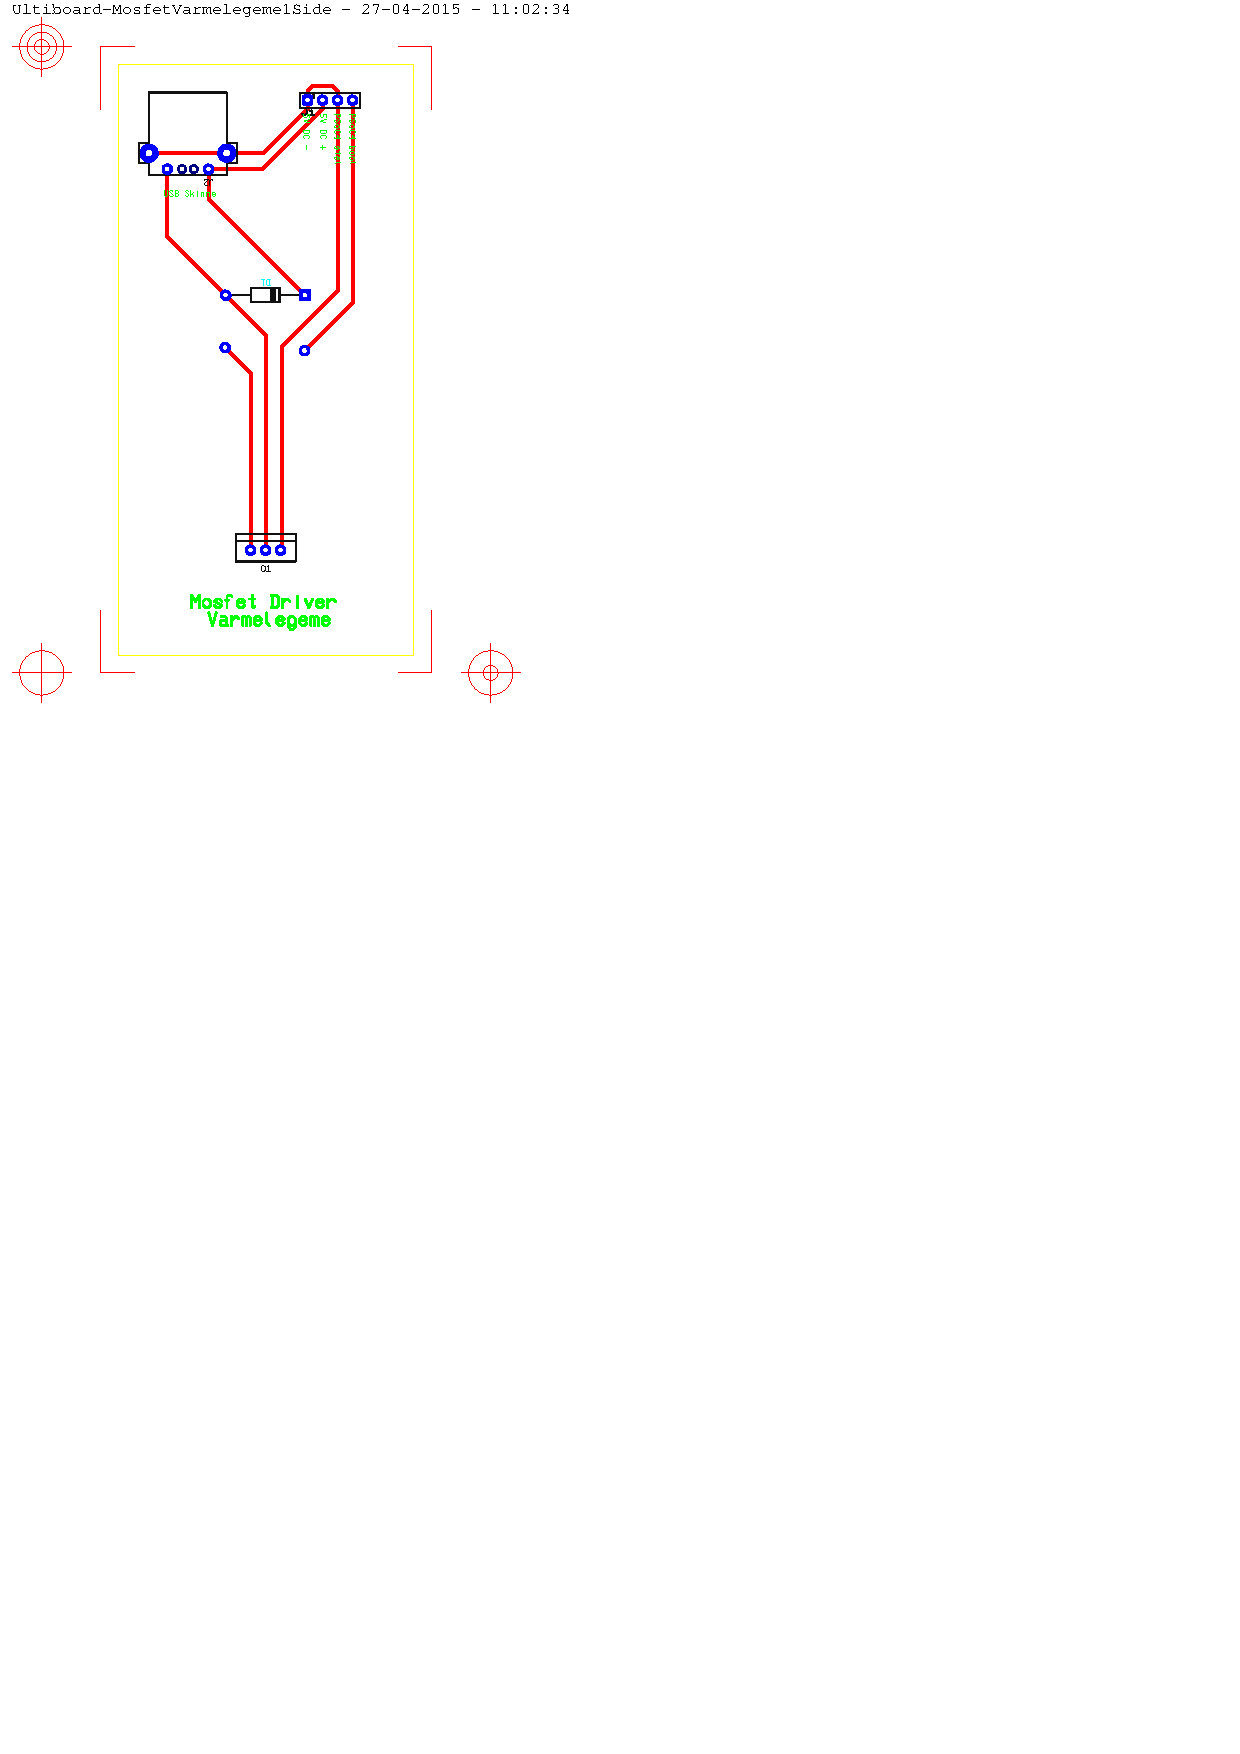
\includegraphics[width={\textwidth-8cm}, trim=50 520 390 30, clip=true, angle =90] {../fig/ultiboard_varmelegeme.pdf}
\caption{Printudlæg for Mosfet driver til Varmelegeme i Ultiboard}
\label{fig:ultiboard_varmelegeme}
\end{figure}

Implementering af mosfet driveren til varmelegemet foretages ved at Multisim diagrammet eksporteres til Ultiboard, hvorefter printet udlægges.
Det forsøges gjort således at printet er overskueligt fremfor at printet fylder så lidt som muligt. 
Som udgangspunkt er alle forbindelser på printet lagt på bagsiden. 
Det designede print er vist på Figur \ref{fig:ultiboard_varmelegeme}. 

Kobber på undersiden af printet er vist med rød, mens kobber på oversiden af printet er vist med grøn. 
Kobberøer er vist med blå.
Der er en lille hage ved kobberøerne; der er ikke forbindelse mellem oversiden og undersiden. 
Dette har dog ingen betydning, da der loddes komponentben igennem dem alle. 

Omkredserne af komponenterne (sort) printes ikke, de vises kun som en slags hjælpelag. 

Databasen i Ultiboard indeholder ikke komponenter til modstande, derfor er disse omkredse ikke med på figuren. 

Der skrives lidt forklarende tekst på oversiden af printet, så man kan se hvad der skal kobles til hvor; dette er lidt svært at se på figuren.
\newline

Printudlægget bestilles ved E-LAB på IHA, hvorefter komponenter loddes på.
Det færdige print er vist på Figur \ref{fig:varmelegeme_print}.

\begin{figure}[h]
\centering 
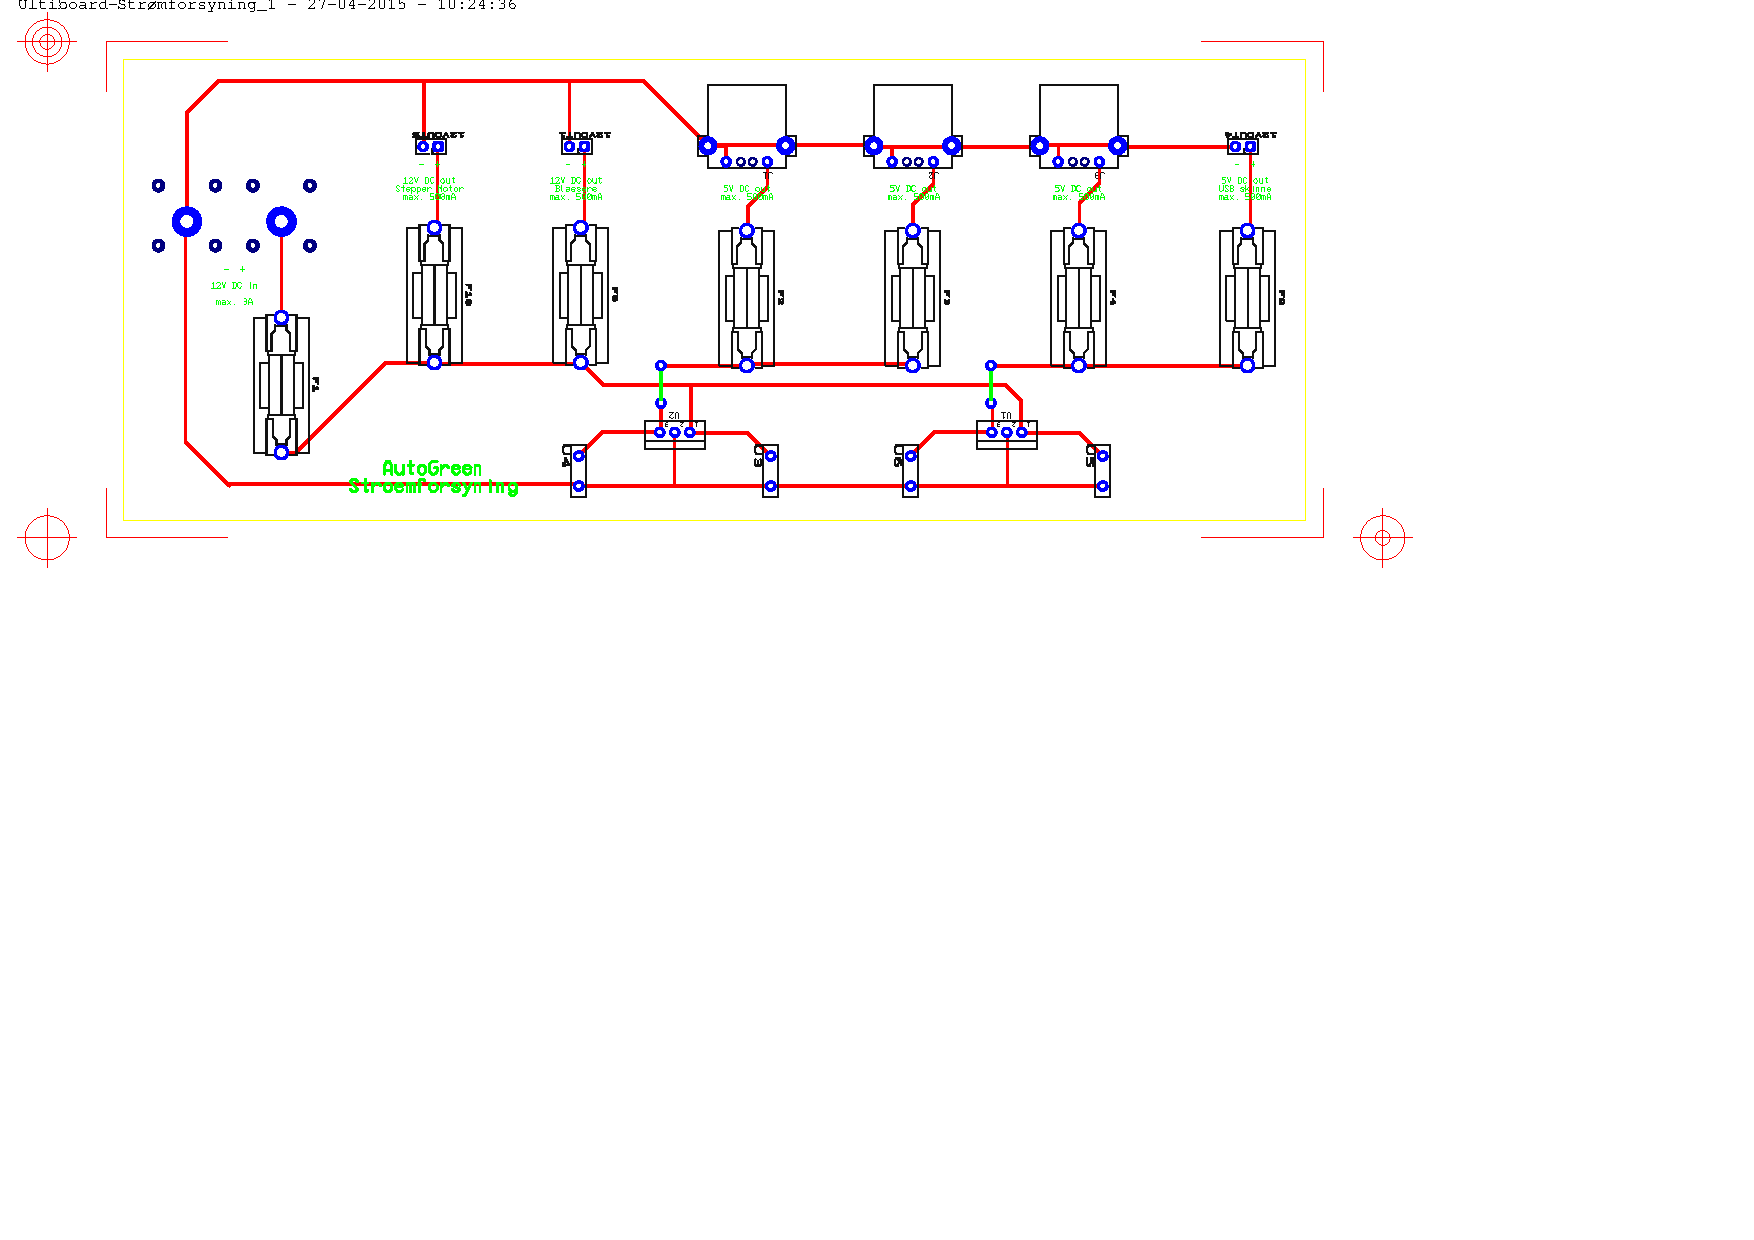
\includegraphics[width={\textwidth}, trim=0 0 0 0, clip=true] {../fig/ultiboard_stroemforsyning.pdf} %TODO Indsæt billede af det færdige print.
\caption{Den færdige Mosfet driver til Varmelegeme}
\label{fig:varmelegeme_print}
\end{figure}

\clearpage

\subsection{HW Blæsere}

Implementering af Mosfetdriver til Blæsere foretages på samme måde som til Varmelegeme.
Printudlægget i Ultiboard er vist på Figur \ref{fig:ultiboard_blaesere}, og det færdige print er vist på Figur \ref{fig:blaesere_print}.

\begin{figure}[h]
\centering 
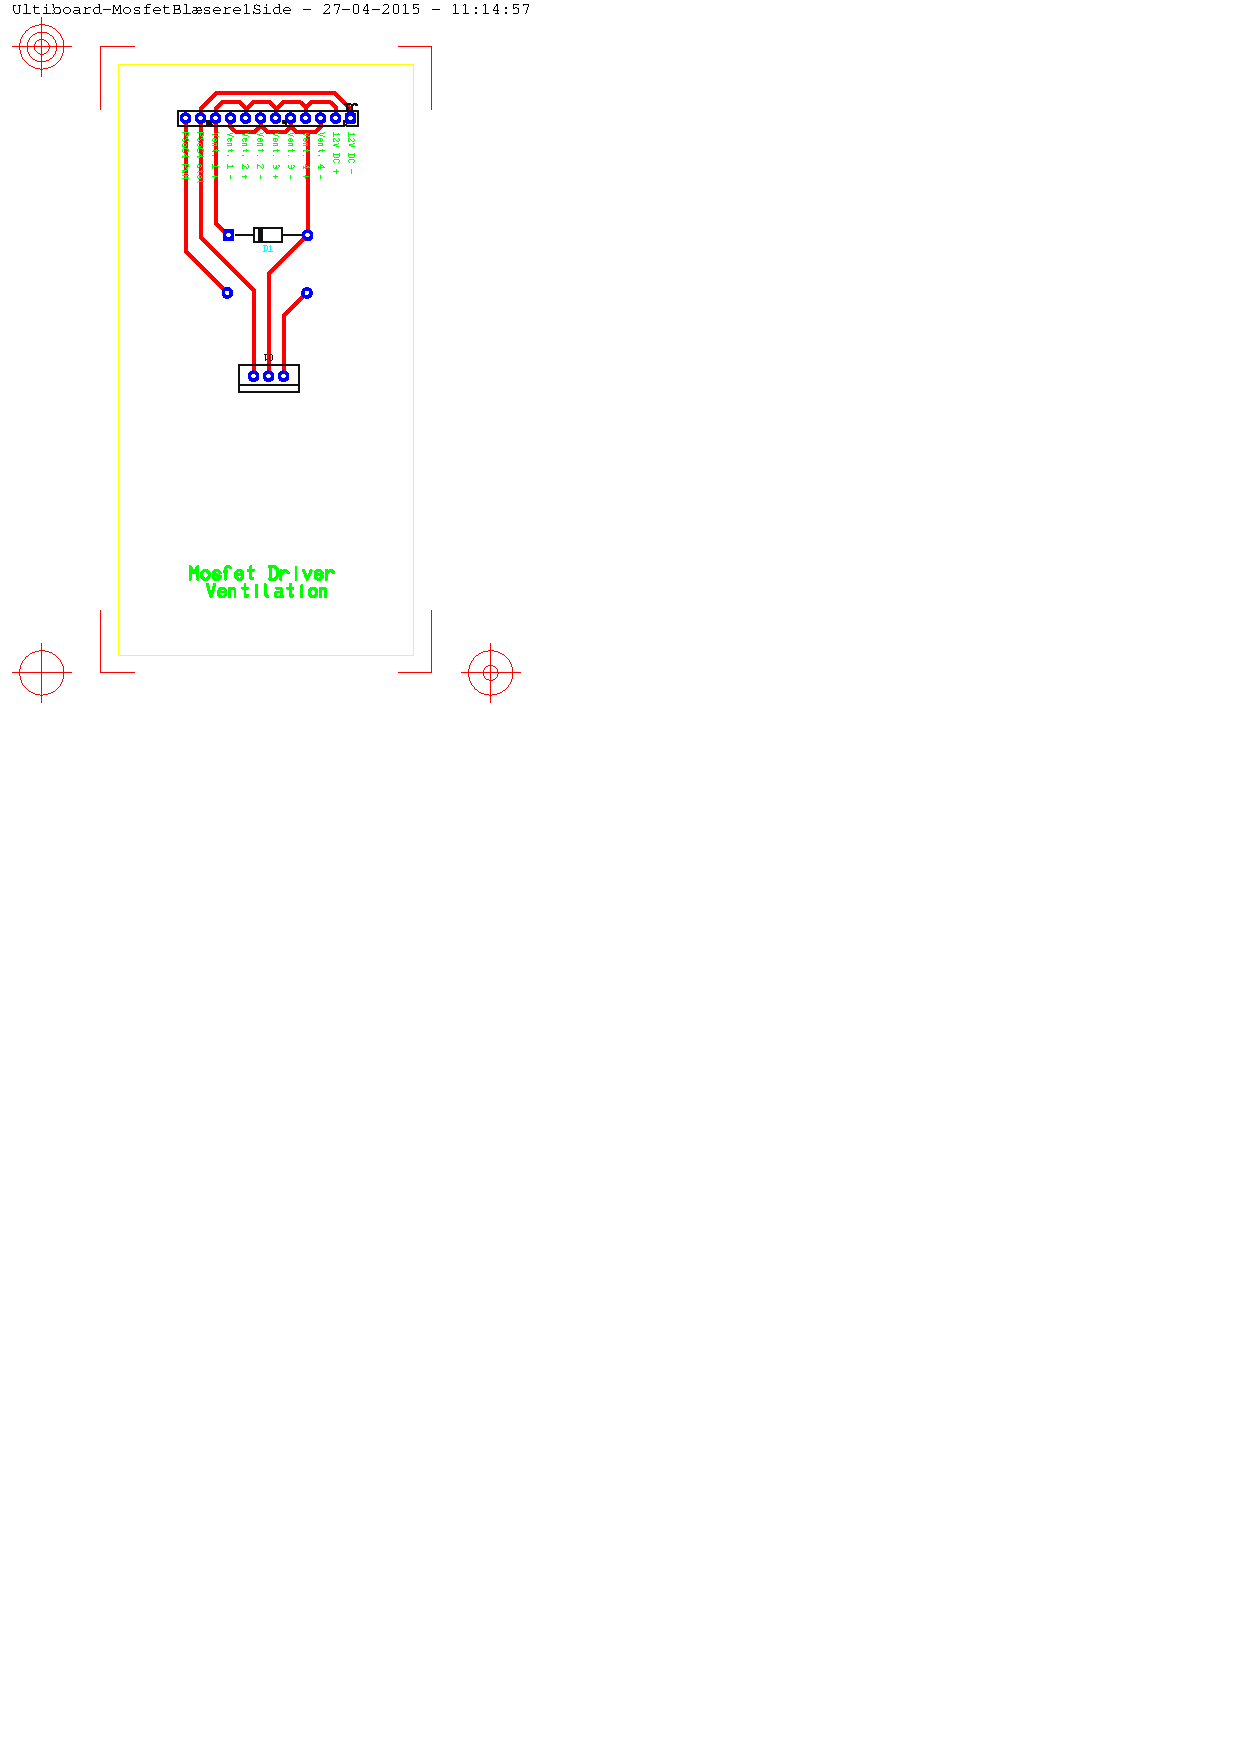
\includegraphics[width={\textwidth-8cm}, trim=50 520 390 30, clip=true, angle =90] {../fig/ultiboard_blaesere.pdf}
\caption{Printudlæg for Mosfet driver til Blæsere i Ultiboard}
\label{fig:ultiboard_blaesere}
\end{figure}

\begin{figure}[h]
\centering 
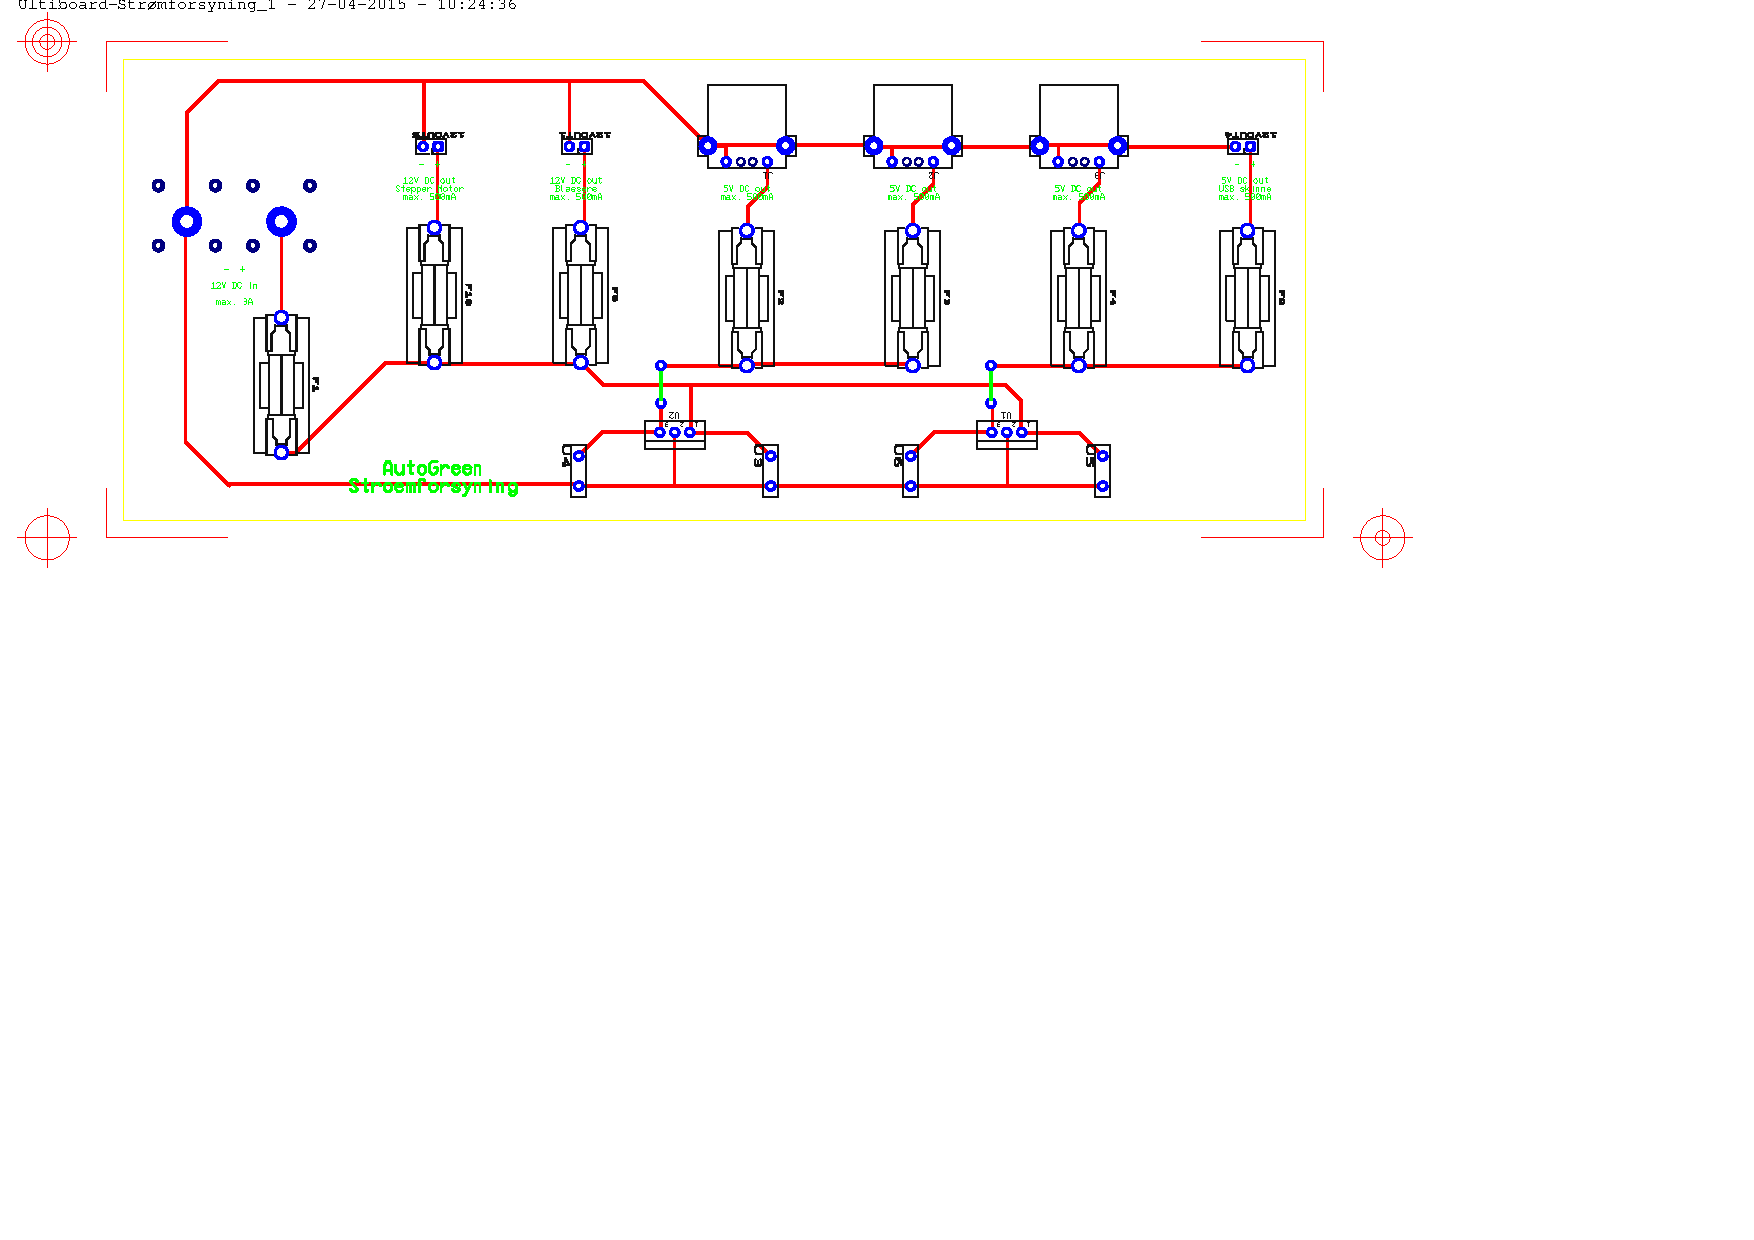
\includegraphics[width={\textwidth}, trim=0 0 0 0, clip=true] {../fig/ultiboard_stroemforsyning.pdf} %TODO Indsæt billede af det færdige print.
\caption{Den færdige Mosfet driver til Blæsere}
\label{fig:blaesere_print}
\end{figure}

\clearpage

\subsection{HW Vinduesmotor}

Implementering af Mosfetdriver til Vinduesmotor foretages på samme måde som til Varmelegeme og Blæsere.
Printudlægget i Ultiboard er vist på Figur \ref{fig:ultiboard_vinduesmotor}, og det færdige print er vist på Figur \ref{fig:vinduesmotor_print}. %TODO

\begin{figure}[h]
\centering 
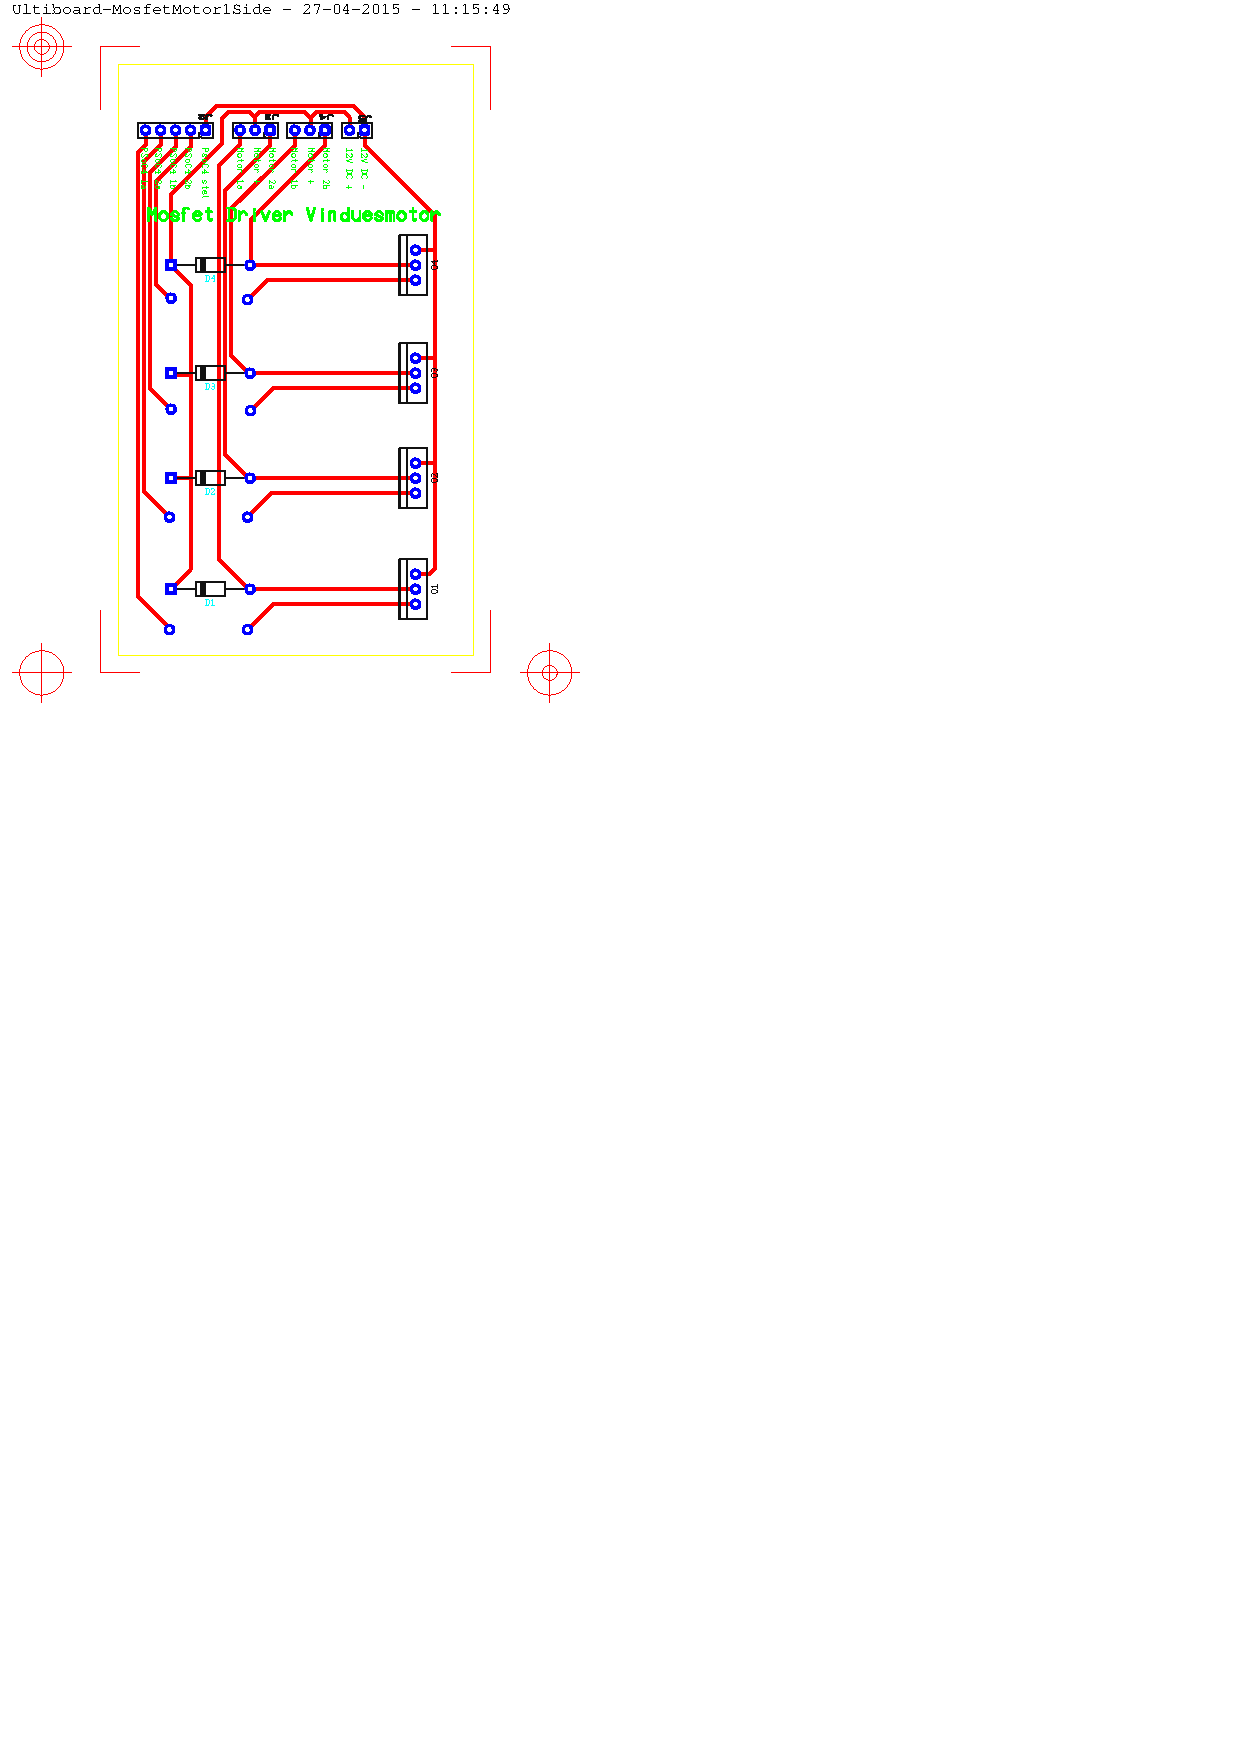
\includegraphics[width={\textwidth-6cm}, trim=50 520 365 30, clip=true, angle =90] {../fig/ultiboard_vinduesmotor.pdf} %TODO
\caption{Printudlæg for Mosfet driver til Vinduesmotor i Ultiboard}
\label{fig:ultiboard_vinduesmotor}
\end{figure}

\begin{figure}[h]
\centering 
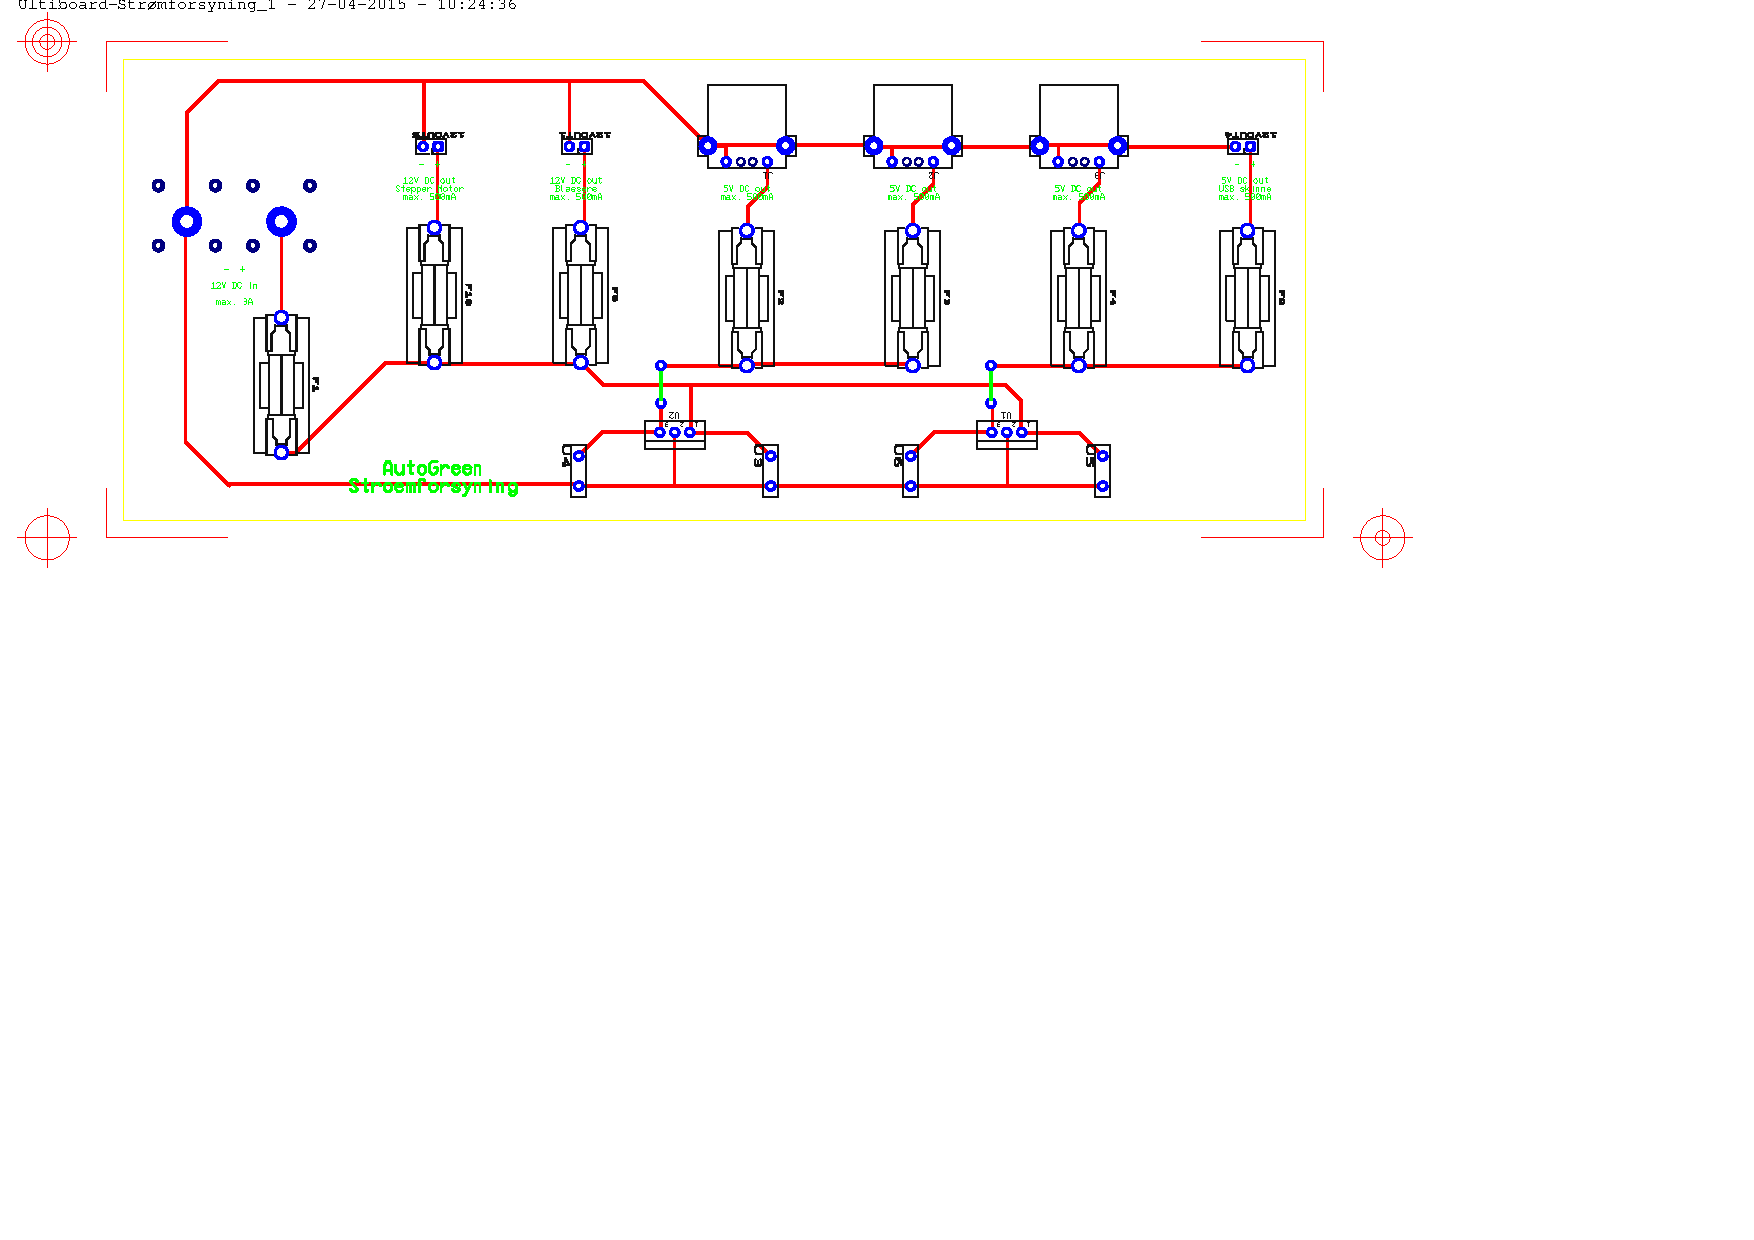
\includegraphics[width={\textwidth}, trim=0 0 0 0, clip=true] {../fig/ultiboard_stroemforsyning.pdf} %TODO Indsæt billede af det færdige print.
\caption{Den færdige Mosfet driver til Vinduesmotor}
\label{fig:vinduesmotor_print}
\end{figure}

\clearpage